\documentclass{beamer}
% \documentclass[handout]{beamer}

% \usetheme{Antibes}
% \usetheme{Berlin}
\usetheme{CambridgeUS}
% \usetheme{Copenhagen}

\usepackage{hyperref}
\usepackage{caption}
\usepackage{ytableau}
\usepackage{tikz-cd}
\usepackage{centernot}
\usepackage[shortlabels]{enumitem}
\usepackage{cases}
\usepackage{bbm}

\usepackage{booktabs}

\usetikzlibrary{shadows}

\newtheorem{thm}{Theorem}[section]
\newtheorem{FermatLastTheorem}{Fermat's Last Theorem}[section]
\newtheorem{IMO_P2}{IMO 2024 Problem 2}[section]
\newtheorem{lem}[thm]{Lemma}
\newtheorem{prop}[thm]{Proposition}
\newtheorem{cor}[thm]{Corollary}
\newtheorem{conj}[thm]{Conjecture}
\newtheorem*{conj1}{Conjecture 1}
\newtheorem*{conj2}{Conjecture 2}
\newtheorem*{conj3}{Conjecture 3}
\theoremstyle{definition}
\newtheorem{exam}[thm]{Example}
\newtheorem{prob}[thm]{Problem}
\newtheorem{defn}[thm]{Definition}
\newtheorem{assumption}{Assumption}
\newtheorem{todo}{To-Do}
\newtheorem{remark}[thm]{Remark}

\newcommand\asc{\operatorname{asc}}
\newcommand\des{\operatorname{des}}
\newcommand\inv{\operatorname{inv}}
\newcommand\inc{\operatorname{inc}}
\newcommand\sgn{\operatorname{sgn}}
\newcommand\sh{\operatorname{sh}}
\newcommand\rk{\operatorname{rank}}
\newcommand\lex{\operatorname{lex}}
\newcommand\row{\operatorname{row}}
\newcommand\col{\operatorname{col}}
%% \newcommand\deg{\operatorname{deg}}
\newcommand\ch{\operatorname{ch}}
\newcommand\Red{\operatorname{Red}}
\newcommand\plac{\operatorname{plac}}
\newcommand\nCox{\operatorname{nCox}}

\newcommand\Des{\operatorname{Des}}
\newcommand\SYT{\operatorname{SYT}}
\newcommand\SSYT{\operatorname{SSYT}}
\newcommand\Par{\operatorname{Par}}
\newcommand\Comp{\operatorname{Comp}}

\newcommand\Ind{\operatorname{Ind}}

\newcommand\GL{\operatorname{GL}}
\newcommand\gl{\mathfrak{gl}}

\newcommand\NSym{\mathsf{NSym}}
\newcommand\Sym{\mathsf{Sym}}
\newcommand\QSym{\mathsf{QSym}}

\newcommand\gge{\succcurlyeq}
\newcommand\lle{\preccurlyeq}
\newcommand\trigeq{\unrhd}
\newcommand\trileq{\unlhd}

\newcommand\TT{\mathcal{T}}
\newcommand\UU{\mathcal{U}}
\newcommand\EE{\mathcal{E}}
\newcommand\SSS{\mathcal{S}}
\newcommand\II{\mathcal{I}}
\newcommand\LL{\mathcal{L}}
\newcommand\HH{\mathcal{H}}
\newcommand\SYM{\mathfrak{S}}

\newcommand\ZZ{\mathbb{Z}}
\newcommand\NN{\mathbb{N}}
\newcommand\QQ{\mathbb{Q}}
\newcommand\CC{\mathbb{C}}

\newcommand\xx{\mathbf{x}}
\newcommand\yy{\mathbf{y}}
\newcommand\uu{\mathbf{u}}
\newcommand\mm{\mathbf{m}}

\newcommand\ee{\mathfrak{e}}
\newcommand\hh{\mathfrak{h}}
\newcommand\ff{\mathfrak{f}}
\newcommand\sch{\mathfrak{s}}
\newcommand\pp{\mathfrak{p}}
\newcommand\mono{\mathfrak{m}}
\newcommand\FF{\mathfrak{F}}
\newcommand\MM{\mathfrak{M}}

\newcommand\ww{\mathsf{w}}
\newcommand\vv{\mathsf{v}}
\newcommand\zz{\mathsf{z}}

\newcommand\oo{\mathfrak{o}}



\newcommand\equivclass[1]{#1/{\sim}}
\newcommand\qand{\quad\mbox{and}\quad}
\newcommand\mand{\mbox{ \& }}
\newcommand{\precdot}{\prec\mathrel{\mkern-5mu}\mathrel{\cdot}}

\newcommand\CHK[1]{\textcolor{red}{#1}}
\newcommand\RED[1]{\textcolor{red}{#1}}
\newcommand\remph[1]{\emph{\textcolor{red}{#1}}}
\newcommand\bemph[1]{\emph{\textcolor{blue}{#1}}}



\title{FunSearch: doing mathematics via LLM}
\author[Byung-Hak Hwang]{Byung-Hak Hwang}
\institute[KIAS]{KIAS}
\date[]{Winter School on Math+AI \\ November 12, 2025}

%%%%%%%%%%%%%%%%%%%%%%%%%%%%%%%%%%%%%%%%%%%%%%

\AtBeginSection[]{%
\begin{frame}
    \tableofcontents[currentsection, subsectionstyle=show/show/hide]
\end{frame}
}

%%%%%%%%%%%%%%%%%%%%%%%%%%%%%%%%%%%%%%%%%%%%%%

\makeatletter
\let\save@measuring@true\measuring@true
\def\measuring@true{%
  \save@measuring@true
  \def\beamer@sortzero##1{\beamer@ifnextcharospec{\beamer@sortzeroread{##1}}{}}%
  \def\beamer@sortzeroread##1<##2>{}%
  \def\beamer@finalnospec{}%
}
\makeatother

%%%%%%%%%%%%%%%%%%%%%%%%%%%%%%%%%%%%%%%%%%%%%%

\makeatletter
\newenvironment<>{proofs}[1][\proofname]{%
    \par
    \def\insertproofname{#1\@addpunct{.}}%
    \usebeamertemplate{proof begin}#2}
  {\usebeamertemplate{proof end}}
\newenvironment<>{proofc}{%
  \setbeamertemplate{proof begin}{\begin{block}{}}
    \par
    \usebeamertemplate{proof begin}}
  {\usebeamertemplate{proof end}}
\newenvironment<>{proofe}{%
    \par
    \pushQED{\qed}
    \setbeamertemplate{proof begin}{\begin{block}{}}
    \usebeamertemplate{proof begin}}
  {\popQED\usebeamertemplate{proof end}}
\makeatother

%%%%%%%%%%%%%%%%%%%%%%%%%%%%%%%%%%%%%%%%%%%%%%


\begin{document}

\begin{frame}
  \titlepage
\end{frame}

\begin{frame}
  \frametitle{AI for Math}
  \begin{itemize}
    \item \textbf{AI for Math} aims to use machine learning models to assist or automate mathematical reasoning and discovery. \vspace{.3cm}
    \item Recent advances in \textbf{LLMs} (large language models) and \textbf{generative models} have shown potential not only in theorem proving but also in finding new mathematical constructions. \vspace{.3cm}
    \item These approaches shift the focus from ``solving problems directly'' to ``searching for algorithms or functions'' that generate valid and sometimes novel results.
  \end{itemize}
\end{frame}

\begin{frame}
  \begin{center}
    \begin{tabular}{|p{3.4cm}|p{2.5cm}|p{3.2 cm}|}
      \toprule
      \textbf{Pattern recognizer} & \textbf{Code agent} & \textbf{Automated theorem prover} \\
      \midrule
      Own model \newline for each problem \newline (Transformer, GNN, RL, etc.)
        & FunSearch,\newline AlphaEvolve
        & AlphaProof,\newline Gemini Deep Think,\newline Aristotle \\
      \midrule
      Hypercube decomposition,\newline Murmuration
        & Cap Set,\newline Isosceles-free Set
        & Gold-medal\newline performance at IMO \\
      \bottomrule
    \end{tabular}
  \end{center}
\end{frame}

\begin{frame}
  \frametitle{FunSearch}
  \begin{itemize}
    \item \textbf{FunSearch} (short for “searching in the function space”) was developed by Google DeepMind~\cite{RBNBKDREWFKF2024}. \vspace{.3cm}
    \item It combines a pretrained LLM (creative component) with an \textbf{evaluator} (rigorous verifier). \vspace{.3cm}
    \item FunSearch evolves programs through an \textbf{LLM-driven genetic algorithm}. \vspace{.3cm}
    \item This process iteratively improves “programs that solve the problem,” not just their outputs.
  \end{itemize}
\end{frame}

\begin{frame}
  \frametitle{FunSearch}
  \begin{center}
    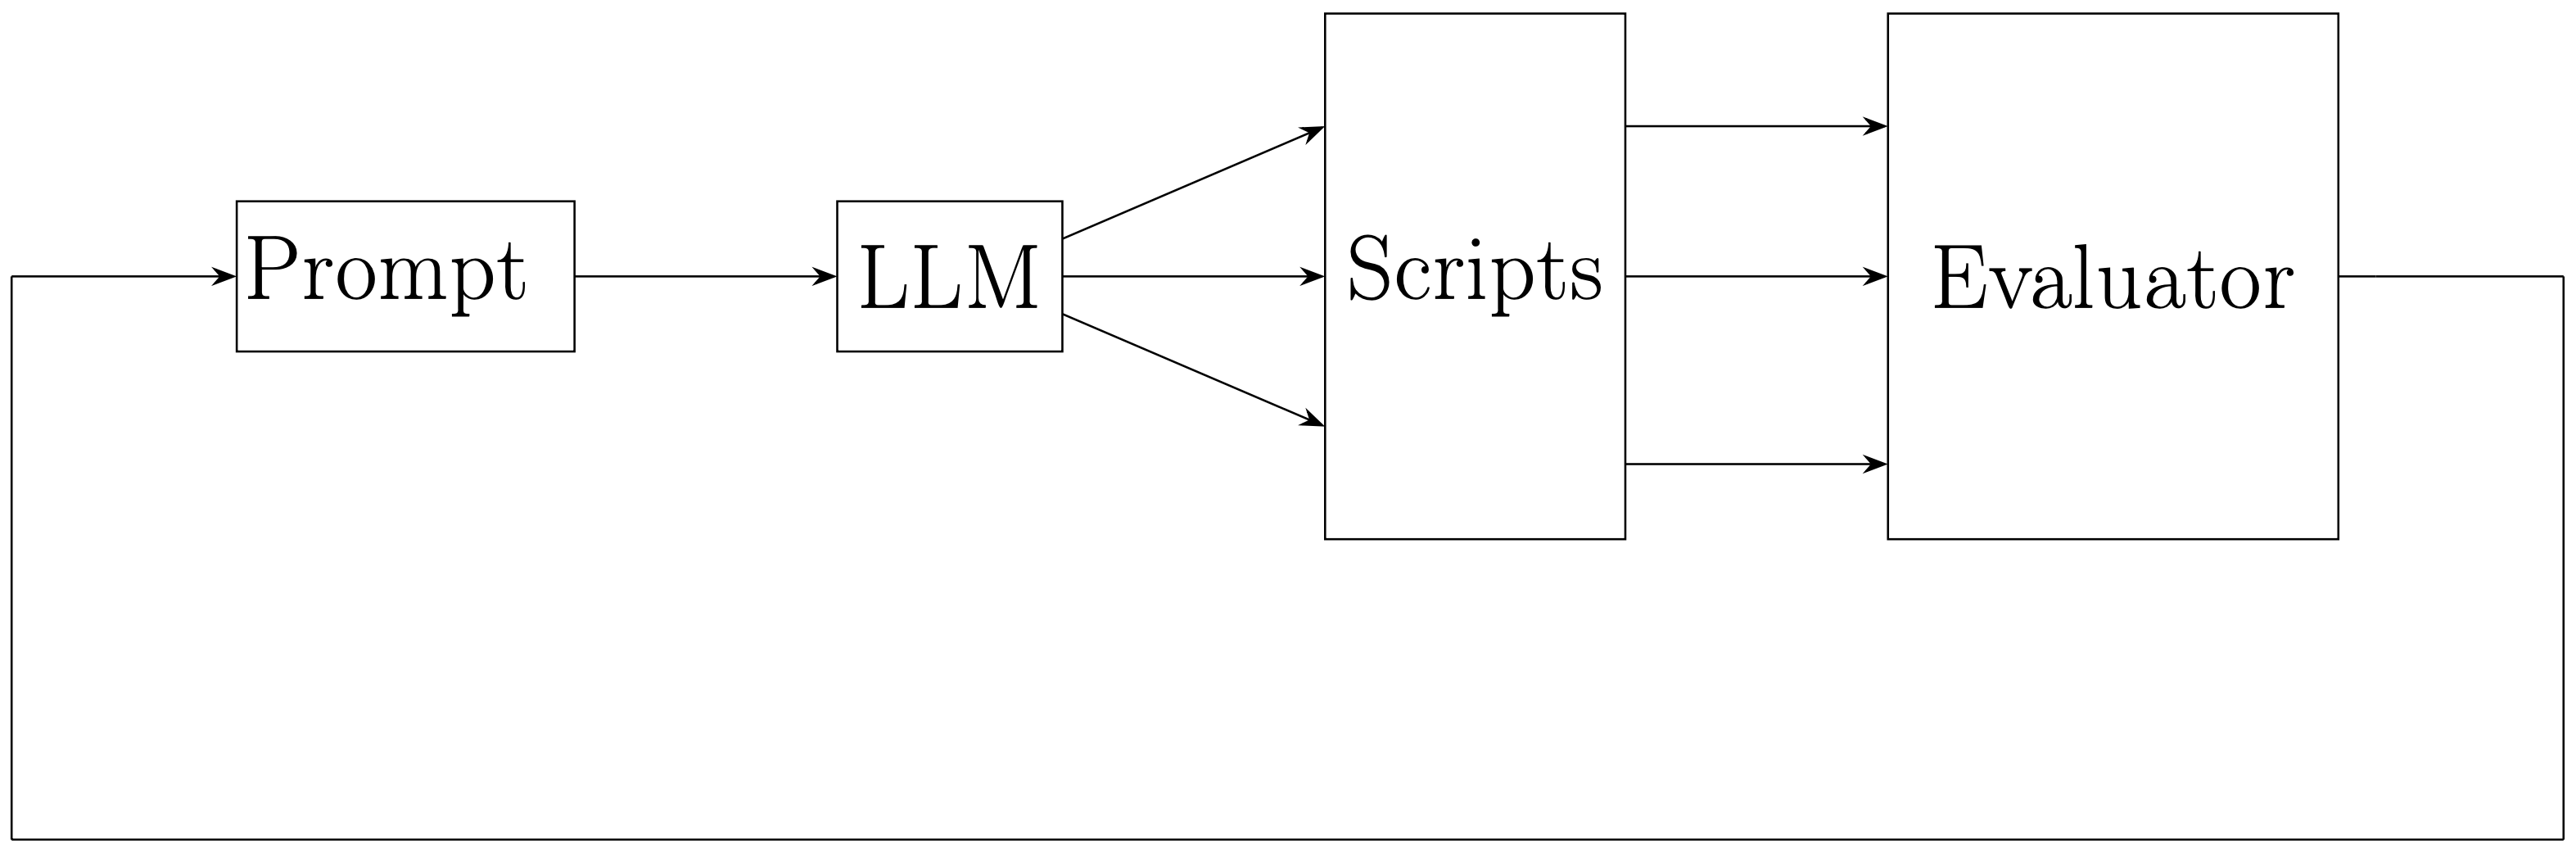
\includegraphics[scale=.2]{./figures/Workflow.png} \\
    A workflow of FunSearch (captured from \cite{EFHSS2025})
  \end{center}
  \begin{enumerate}[label=(\roman*)]
  \item Generate candidate programs (Python functions).  
  \item Evaluate their performance on the target problem.  
  \item Feed the best (and diverse) candidates back to the LLM prompt.  
  \item The LLM produces new variants—forming the next generation.  
\end{enumerate}
\end{frame}

\begin{frame}
  \frametitle{What problems FunSearch can handle}
  \begin{itemize}
    \item Problems that are easy to evaluate but hard to solve directly. \vspace{.3cm}
    \item Especially suited for:
      \begin{itemize}
        \item Extremal or additive combinatorics (e.g., Cap Set problem)
        \item Number theory problems with clear scoring metrics
        \item Combinatorial optimization (e.g., Bin packing)
      \end{itemize} \vspace{.3cm}
    \item Requires problems where the evaluation function is deterministic and computationally feasible. \vspace{.3cm}
    \item FunSearch discovers \emph{heuristics or algorithms}, not full proofs.
  \end{itemize}
\end{frame}

\begin{frame}
  The following is the list of the problems considered in the paper: \vspace{.2cm}
  \begin{itemize}
    \item[$\bullet$] Cap Set problem (extremal combinatorics)
    \item[$\bullet$] Online bin packing (algorithmic optimization)  
    \item[$\bullet$] Narrow admissible tuples (analytic number theory)  
    \item[$\bullet$] No-isosceles subset of a grid (geometric combinatorics)  
    \item[$\bullet$] (Supplementary) Corners problem and Shannon capacity of cycle graphs
  \end{itemize}
\end{frame}

\begin{frame}
  \frametitle{Example: Cap Set problem}
  \begin{itemize}
    \item The \textbf{Cap Set problem}: find the largest subset of $(\mathbb{Z}/3\mathbb{Z})^n$ containing no three elements whose sum is zero. \vspace{.3cm}
    \item Exact values are known only for $n \le 6$, and the search space grows exponentially. \vspace{.3cm}
    \item FunSearch discovered a new construction in dimension 8, producing a cap set of size 512—the largest known—improving the record for the first time in 20 years. \vspace{.3cm}
    \item Importantly, it found not only the set itself but a \emph{program} that generates it.
  \end{itemize}
\end{frame}

\begin{frame}
  \frametitle{Example: Cap Set problem}
  \begin{center}
    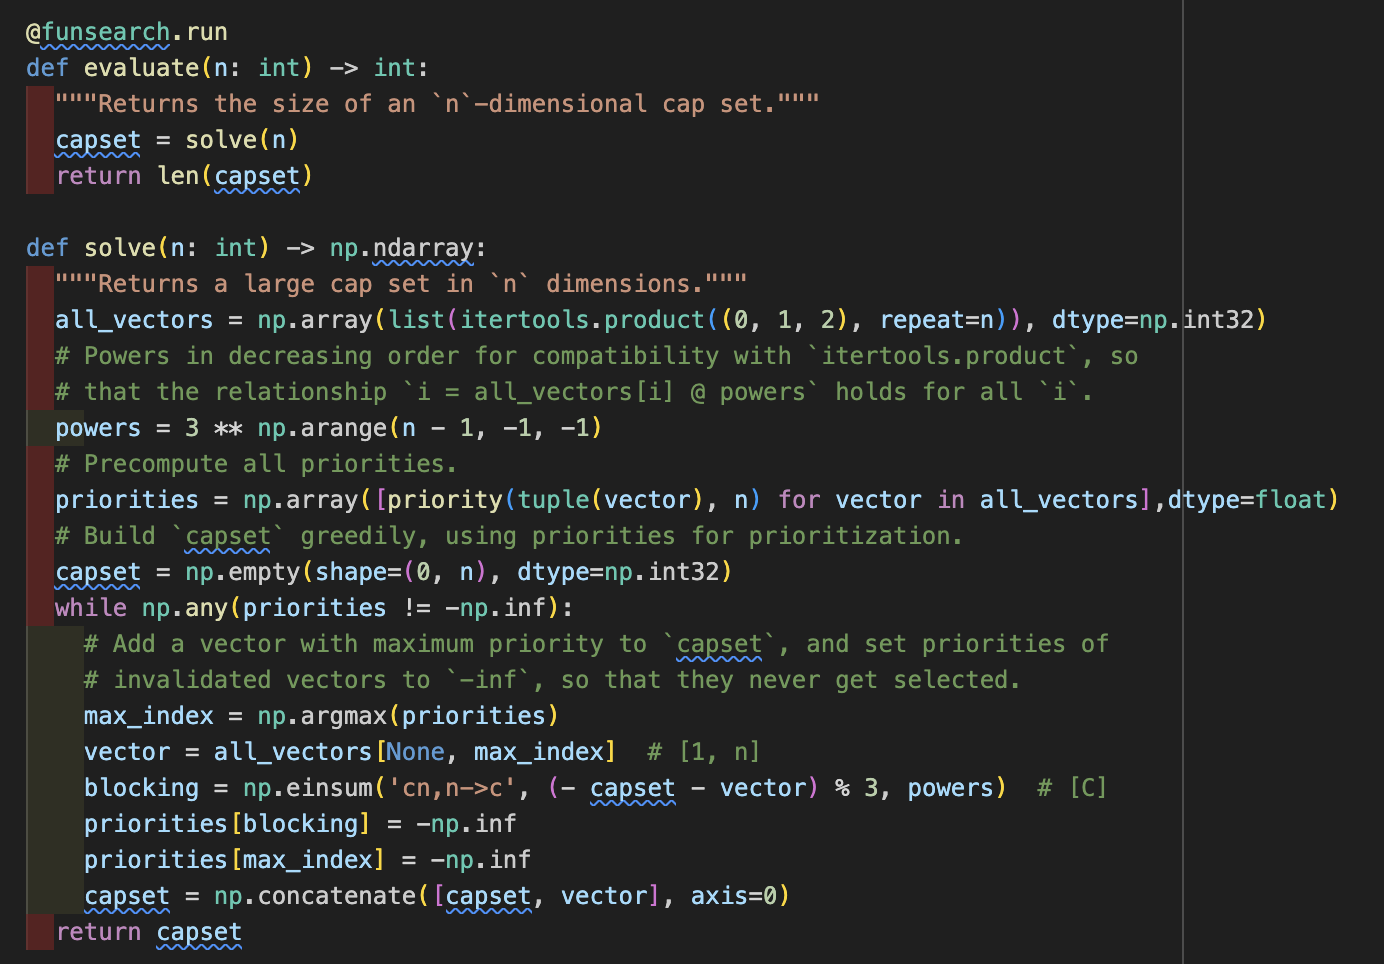
\includegraphics[scale=.4]{./figures/FunSearch_Eval_Solve.png}
  \end{center}
\end{frame}

% \begin{frame}
%   \frametitle{Example: Cap Set problem}
%   \begin{block}{Prompt used in the paper}
%   \scriptsize
%   \begin{verbatim}
%   # Function to be evolved by FunSearch.
%   def priority(element, n):
%     """Returns the priority with which we want
%     to add `element` to the cap set."""
%     return 0.0
%   \end{verbatim}
%   \normalsize
%   \vspace{.3cm}
%   This function is initialized as trivial and evolved through multiple LLM–evaluation loops
%   to learn effective heuristics for building large cap sets.
%   \end{block}
% \end{frame}

\begin{frame}
  \frametitle{Example: Cap Set problem}
  \begin{center}
    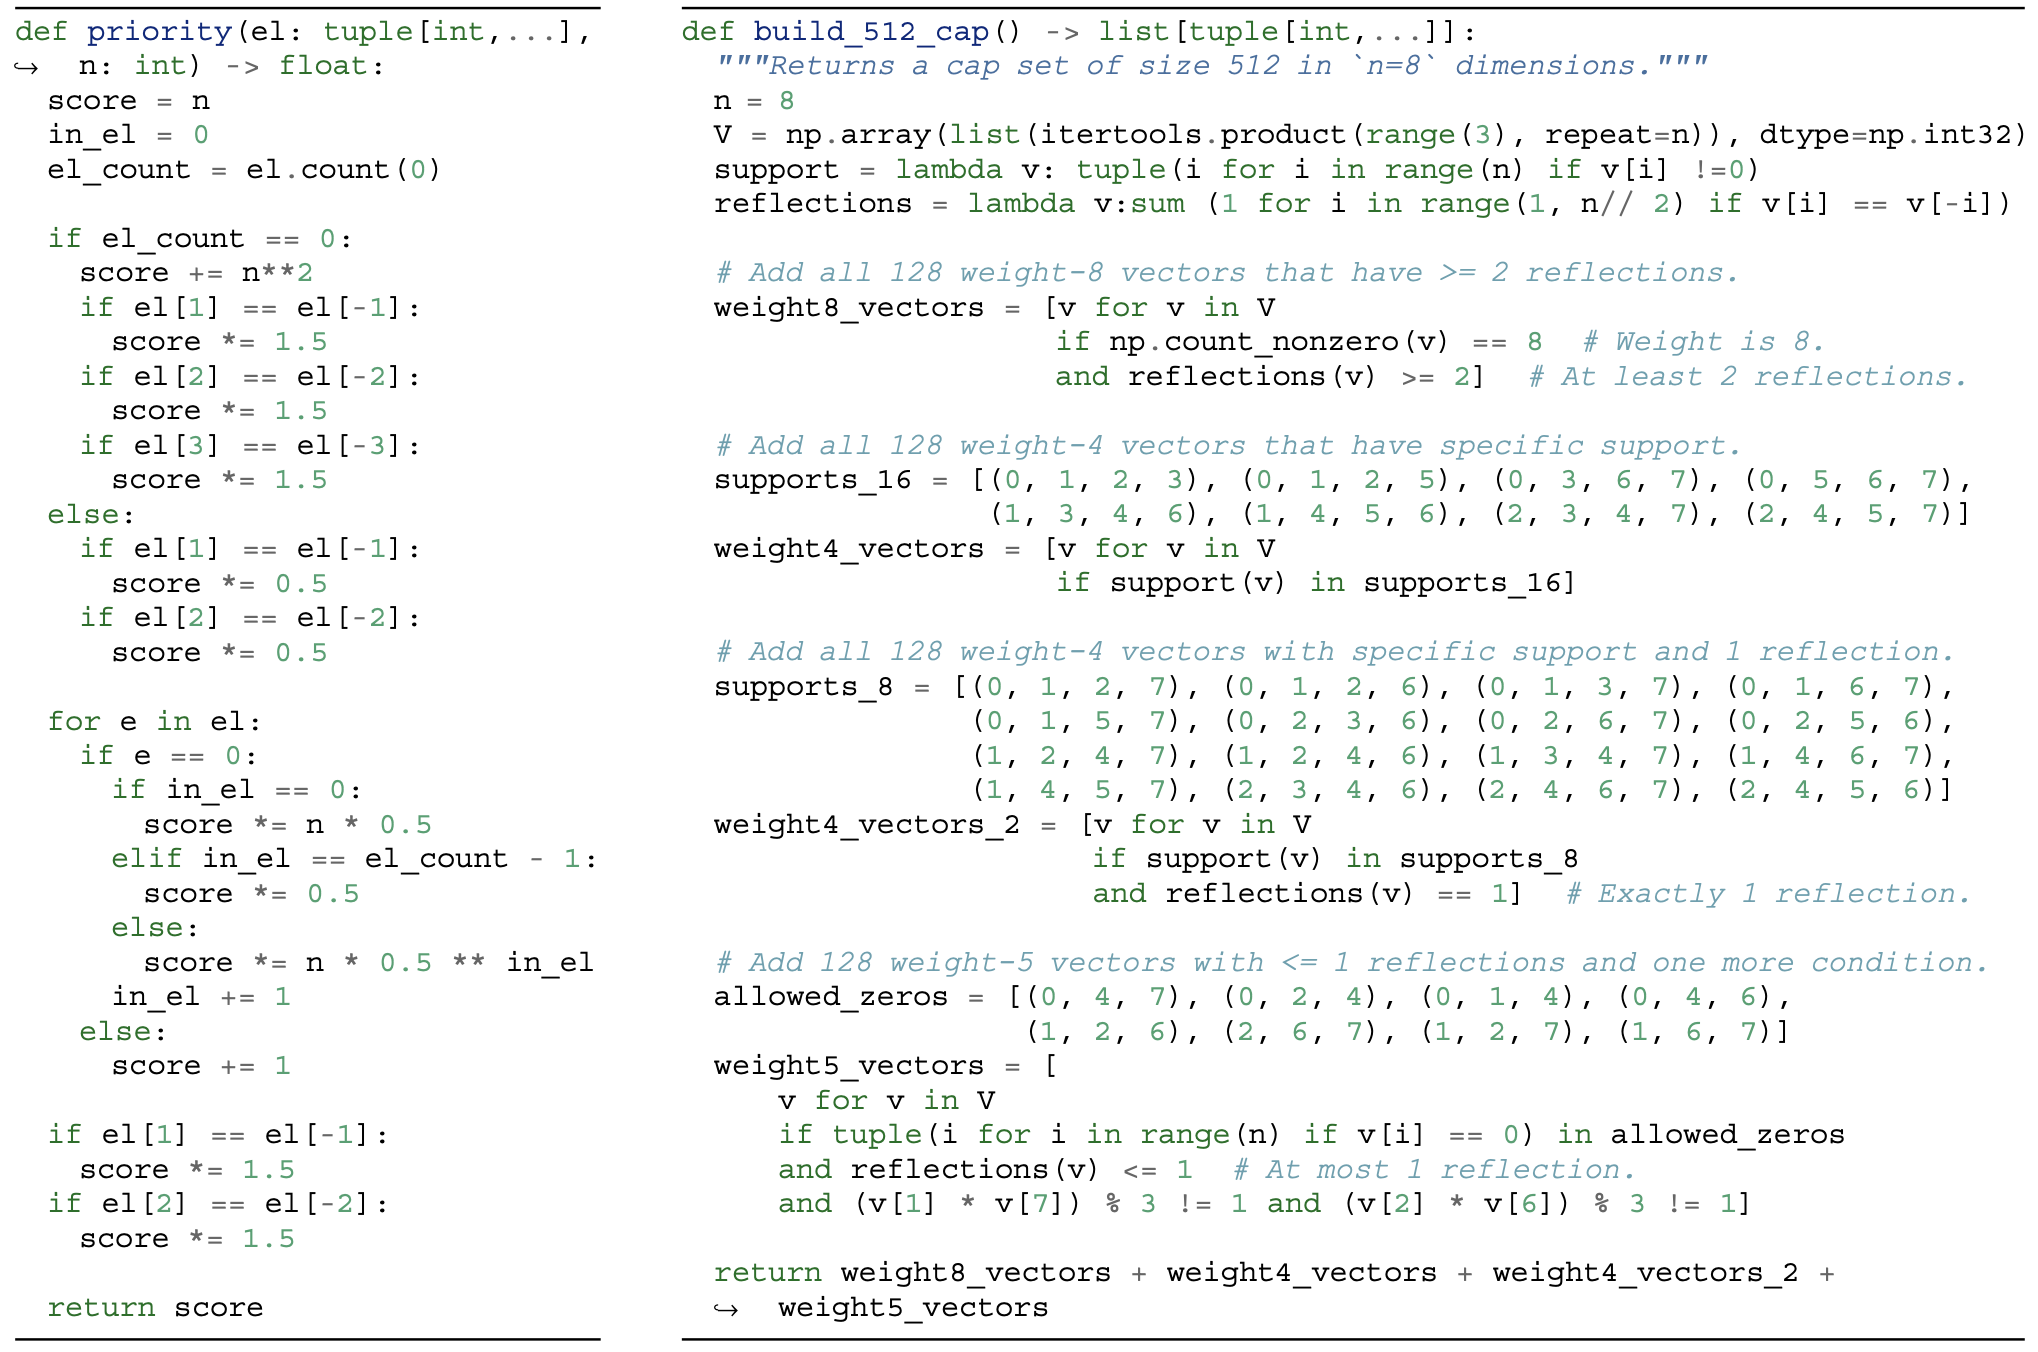
\includegraphics[scale=.3]{./figures/cap_set_priority.png}
  \end{center}
\end{frame}

\begin{frame}
  \frametitle{Example: Cap Set problem}
  \begin{center}
    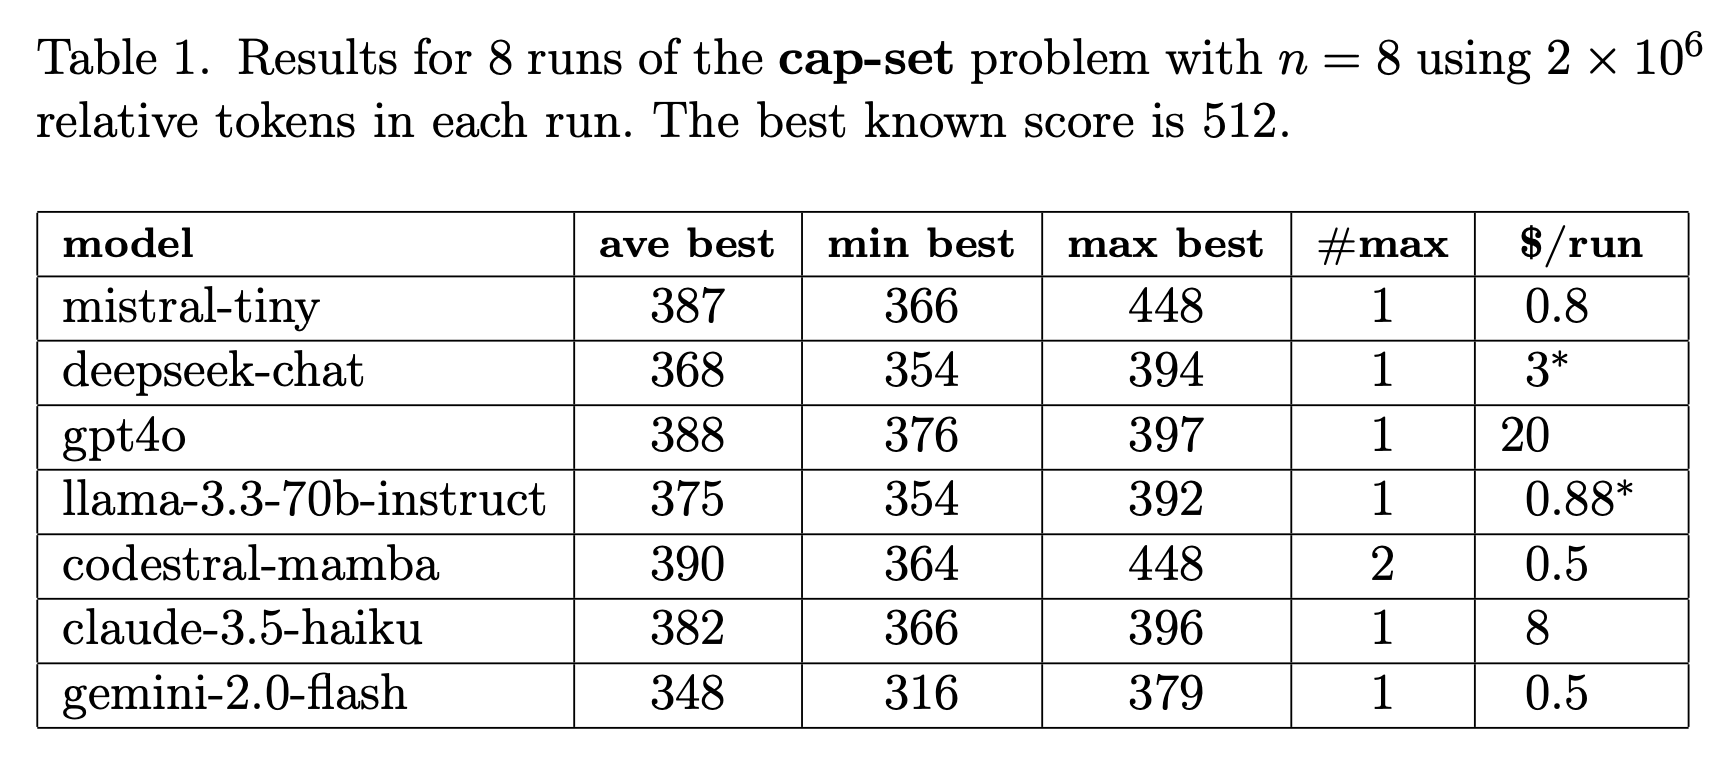
\includegraphics[scale=.385]{./figures/cap_set_API_price.png}
  \end{center}
\end{frame}


\begin{frame}
  \frametitle{Our purposes}
  \begin{enumerate}[label=(\roman*)]
    \item Explore FunSearch with toy examples. \vspace{.3cm}
    \item Refine the methods of applying FunSearch described in the papers. \vspace{.3cm}
    \item Apply FunSearch to other problems in discrete mathematics. 
  \end{enumerate}
\end{frame}

\begin{frame}
  \begin{itemize}
    \item[\( \bullet \)] Do you have experience using LLM APIs? \vspace{.3cm}
    \item[\( \bullet \)] Do you have some computing resources? \vspace{.3cm}
    \item[\( \bullet \)] Are you familiar with Python programming? \vspace{.3cm}
    \item[\( \bullet \)] Do you know any problems in discrete mathematics that could be tackled with FunSearch?
  \end{itemize}
\end{frame}

\section*{}
\begin{frame}
\begin{center}
\Huge{Questions?}
\end{center}
\end{frame}

\begin{frame}
  \frametitle{References}
  \bibliographystyle{alpha}
  \bibliography{/Users/hwangbyunghak/Documents/newbiemacs/nbm-user-settings/references/ref.bib}
\end{frame}


\end{document}